\documentclass[11pt]{article}

\usepackage[preprint]{acl}
\usepackage{times}
\usepackage{latexsym}
\usepackage[T1]{fontenc}
\usepackage[utf8]{inputenc}
\usepackage{microtype}
\usepackage{inconsolata}
\usepackage{graphicx}
\usepackage{booktabs}
\usepackage{tabularx}
\usepackage{array}
\usepackage{amsmath}
\usepackage{amssymb}
\usepackage{pifont}
\usepackage{xcolor}
\usepackage{enumitem}
\usepackage{float}
\usepackage{tikz}
\usetikzlibrary{positioning,arrows.meta,calc,fit,backgrounds}

\newcommand{\yes}{\textcolor{okgreen}{\ding{51}}}
\newcommand{\no}{\textcolor{failred}{\ding{55}}}
\newcommand{\partly}{\textcolor{black!55}{$\sim$}}
\newcommand{\na}{\textcolor{black!40}{--}}

\definecolor{okgreen}{RGB}{26,127,55}
\definecolor{failred}{RGB}{176,32,38}
\definecolor{cPrior}{RGB}{118,78,159}   % closed by prior work
\definecolor{cGate}{RGB}{191,128,0}     % gate failed / inconclusive
\definecolor{cConseq}{RGB}{0,118,138}   % true but no consequence
\definecolor{cStd}{RGB}{110,110,110}    % nothing beyond standard tools
\definecolor{cKeep}{RGB}{26,127,55}     % survives as a verified fact

\setlist{nosep,leftmargin=*}
\newcolumntype{L}[1]{>{\raggedright\arraybackslash}p{#1}}
\newcolumntype{Y}{>{\raggedright\arraybackslash}X}
\hypersetup{pdftitle={Proxy Tail: Anatomy of a Failed Research Line on LLM Evaluation in Finance},
  pdfauthor={Letao (Theodore) Ouyang}, pdfkeywords={negative results, post-mortem, LLM evaluation, FinQA, rounding, research process}}

\title{Proxy Tail: Anatomy of a Failed Research Line\\on LLM Evaluation in Finance}

\author{Letao (Theodore) Ouyang \\
  Independent researcher \\
  \texttt{github.com/130U/proxy-tail}}

\begin{document}
\maketitle

\begin{abstract}
Between 15 and 17 November 2026 we ran a research line whose goal was a paper at a top NLP venue. In three days it passed through five stages and four pivots---certified financial language models, tail screening with cheap models, the self-stability of LLM scores, two behavioural probes, and the rounding precision of financial question answering---and it ended with no publishable result. LLM agents executed every experiment under the direction of an LLM advisor; the author set the constraints and made the final calls. This report reconstructs the route, what we believed at each fork, and the evidence that closed each branch. We argue that the failure had one root cause with three faces. A publishable result needs novelty, a consequence that someone cares about, and complete evidence. Agents made evidence cheap, so we produced evidence first and tested novelty and consequence last, although those were the two factors that failed and the two that were cheaper to test. Using the project's own data, we show that each stage could have been closed in hours instead of days, and we turn this into five questions to answer before the first experiment. We also report what survived: a zero-parameter rule that predicts which answers a filing's displayed precision cannot determine (10.7\% of the FinQA test set, confirmed out of sample on TAT-QA), together with the finding that this indeterminacy changes no official score.
\end{abstract}

\section{Introduction}

Most research that fails leaves no trace. The code is deleted, the notes stay private, and the next person with the same idea pays for the same lesson. We think this line is worth writing up for three reasons.

First, it was run in a way that is becoming common: an LLM advisor wrote the research plan and the task briefs, LLM coding agents ran the experiments and wrote most of the notes, and a human set constraints and decided. The work was fast---nine rounds of theory, about 20{,}000 model scores and judgements, and more than 1{,}500 question-level model sessions in three days---and its failure mode is tied to that speed. Second, several negative results are real and reusable: a reference LLM that does not agree with itself in the tail, filings that are self-consistent at their displayed precision, and a benchmark defect that no official score can see. Third, the record is complete. Every task brief, prompt, raw output, pre-registered gate and recomputation is in the repository, so the diagnosis below can be checked rather than taken on trust.

The report makes four contributions:
\begin{itemize}
\item a reconstruction of the route, with what we believed at each fork and why we turned (\S\ref{sec:route}, Figure~\ref{fig:route}, Table~\ref{tab:decisions});
\item a root-cause analysis that separates the proximate cause of each closure from the common cause behind all of them (\S\ref{sec:why});
\item a hindsight audit: for every stage, the earliest signal that could have closed it and the cost of the test that would have read that signal (Table~\ref{tab:audit}), condensed into five questions for next time (\S\ref{sec:lessons});
\item the salvage: the results that did hold up, with their limits (\S\ref{sec:salvage}).
\end{itemize}

\section{Setting}
\label{sec:setting}

\paragraph{People and roles.} The author is a researcher in financial mathematics (certified pricing bounds for path-dependent options, rough-volatility error analysis, and risk bounds under dependence stress). The project had two kinds of AI participants. An \emph{advisor} model (Claude, called ``Fable'' in the repository) proposed directions, wrote task briefs with pre-registered decision rules, and recomputed key numbers before ruling. \emph{Student} agents (OpenAI Codex with GPT-family models, named in the records as \texttt{gpt-6-sol}, \texttt{gpt-6-astra}, \texttt{gpt-6.1-sol}, ``Luna'' and ``Sol'') executed the tasks, scored the items, and wrote most of the reports. Semantic reviews and adjudications in the later stages were also done by AI reviewers. No human annotation was collected.

\paragraph{Constraints.} No GPU beyond free notebook tiers; no model training (decided on the second day); theory first and minimal experiments; and, at the start, no external network access for the student, which was lifted later. The target was one paper at an A-level venue. The project used a strict colour rule: a result counted as publishable only if a novelty check had confirmed it \emph{and} its evidence was complete.

\paragraph{Operating mode.} Each task brief stated one question, the data, the analysis, a pre-registered three-way decision (continue, stop, or inconclusive), and a prior-art step. The student committed raw outputs; the advisor recomputed the main numbers from per-item records before deciding. Tasks were often run in parallel.

\section{The route}
\label{sec:route}

Figure~\ref{fig:route} shows the route and Table~\ref{tab:decisions} gives the reasoning at each fork. We describe each stage by what we asked, what we believed, and what came back.

\begin{figure*}[!t]
\centering
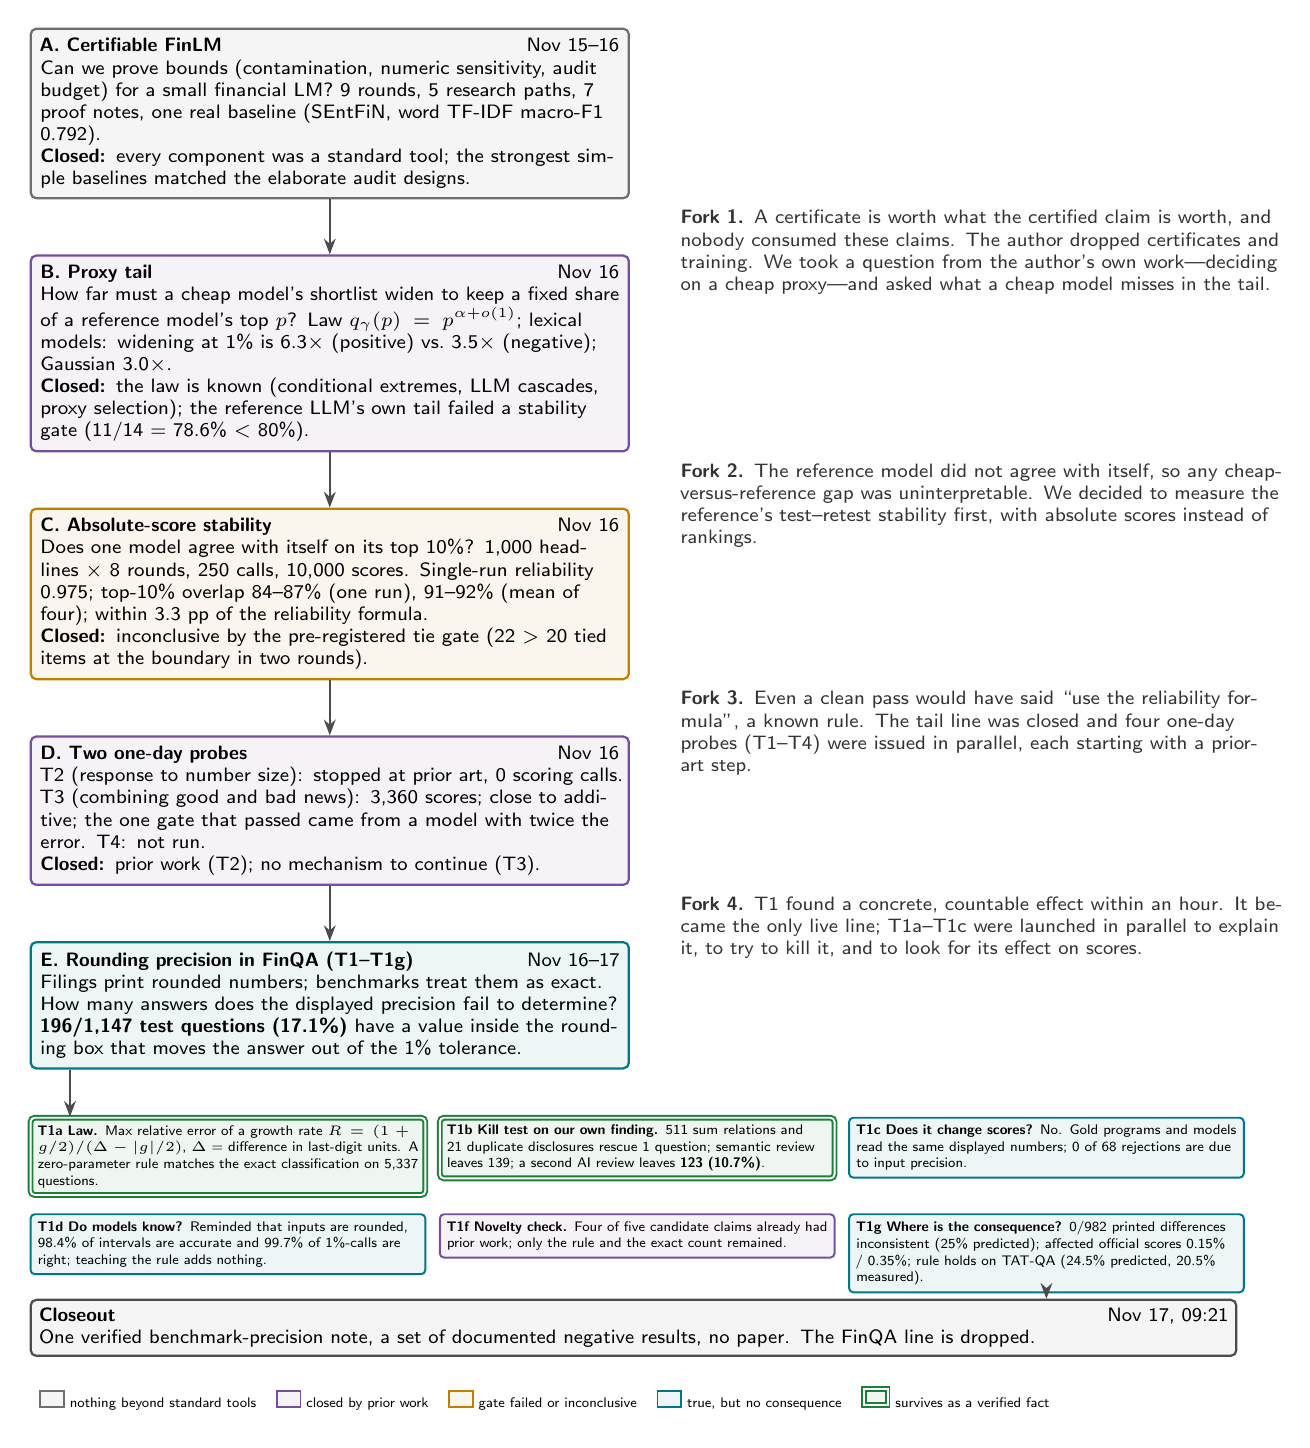
\begin{tikzpicture}[
  font=\sffamily\scriptsize,
  node distance=4mm,
  stage/.style={draw=#1, fill=#1!7, line width=0.8pt, rounded corners=2pt, align=left, text width=7.35cm, inner sep=3.5pt},
  fork/.style={align=left, text width=7.6cm, inner sep=1pt, text=black!80},
  step/.style={draw=#1, fill=#1!7, line width=0.7pt, rounded corners=1.5pt, align=left, text width=4.83cm, inner sep=2.6pt, font=\sffamily\tiny},
  keep/.style={double=white, double distance=0.7pt},
  arr/.style={-{Stealth[length=2mm]}, line width=0.7pt, black!70},
]
\node[stage=cStd] (A) at (0,0) [anchor=north west] {\textbf{A. Certifiable FinLM} \hfill Nov 15--16\\
Can we prove bounds (contamination, numeric sensitivity, audit budget) for a small financial LM?
9 rounds, 5 research paths, 7 proof notes, one real baseline (SEntFiN, word TF-IDF macro-F1 0.792).\\
\textbf{Closed:} every component was a standard tool; the strongest simple baselines matched the elaborate audit designs.};

\node[stage=cPrior, below=7mm of A] (B) {\textbf{B. Proxy tail} \hfill Nov 16\\
How far must a cheap model's shortlist widen to keep a fixed share of a reference model's top $p$?
Law $q_\gamma(p)=p^{\alpha+o(1)}$; lexical models: widening at 1\% is 6.3$\times$ (positive) vs.\ 3.5$\times$ (negative); Gaussian 3.0$\times$.\\
\textbf{Closed:} the law is known (conditional extremes, LLM cascades, proxy selection); the reference LLM's own tail failed a stability gate (11/14 = 78.6\% $<$ 80\%).};

\node[stage=cGate, below=7mm of B] (C) {\textbf{C. Absolute-score stability} \hfill Nov 16\\
Does one model agree with itself on its top 10\%? 1,000 headlines $\times$ 8 rounds, 250 calls, 10,000 scores. Single-run reliability 0.975; top-10\% overlap 84--87\% (one run), 91--92\% (mean of four); within 3.3 pp of the reliability formula.\\
\textbf{Closed:} inconclusive by the pre-registered tie gate (22 $>$ 20 tied items at the boundary in two rounds).};

\node[stage=cPrior, below=7mm of C] (D) {\textbf{D. Two one-day probes} \hfill Nov 16\\
T2 (response to number size): stopped at prior art, 0 scoring calls. T3 (combining good and bad news): 3,360 scores; close to additive; the one gate that passed came from a model with twice the error. T4: not run.\\
\textbf{Closed:} prior work (T2); no mechanism to continue (T3).};

\node[stage=cConseq, below=7mm of D] (E) {\textbf{E. Rounding precision in FinQA (T1--T1g)} \hfill Nov 16--17\\
Filings print rounded numbers; benchmarks treat them as exact. How many answers does the displayed precision fail to determine? \textbf{196/1,147 test questions (17.1\%)} have a value inside the rounding box that moves the answer out of the 1\% tolerance.};

\node[fork, right=6mm of A.south east, anchor=north west, yshift=-1.0mm] (f1) {\textbf{Fork 1.} A certificate is worth what the certified claim is worth, and nobody consumed these claims. The author dropped certificates and training. We took a question from the author's own work---deciding on a cheap proxy---and asked what a cheap model misses in the tail.};
\node[fork, right=6mm of B.south east, anchor=north west, yshift=-1.0mm] (f2) {\textbf{Fork 2.} The reference model did not agree with itself, so any cheap-versus-reference gap was uninterpretable. We decided to measure the reference's test--retest stability first, with absolute scores instead of rankings.};
\node[fork, right=6mm of C.south east, anchor=north west, yshift=-1.0mm] (f3) {\textbf{Fork 3.} Even a clean pass would have said ``use the reliability formula'', a known rule. The tail line was closed and four one-day probes (T1--T4) were issued in parallel, each starting with a prior-art step.};
\node[fork, right=6mm of D.south east, anchor=north west, yshift=-1.0mm] (f4) {\textbf{Fork 4.} T1 found a concrete, countable effect within an hour. It became the only live line; T1a--T1c were launched in parallel to explain it, to try to kill it, and to look for its effect on scores.};

\draw[arr] (A.south) -- (B.north);
\draw[arr] (B.south) -- (C.north);
\draw[arr] (C.south) -- (D.north);
\draw[arr] (D.south) -- (E.north);

% T1 steps
\node[step=cKeep, keep, below=6mm of E.south west, anchor=north west] (a) {\textbf{T1a Law.} Max relative error of a growth rate $R=(1+g/2)/(\Delta-|g|/2)$, $\Delta$ = difference in last-digit units. A zero-parameter rule matches the exact classification on 5,337 questions.};
\node[step=cKeep, keep, right=1.6mm of a.north east, anchor=north west] (b) {\textbf{T1b Kill test on our own finding.} 511 sum relations and 21 duplicate disclosures rescue 1 question; semantic review leaves 139; a second AI review leaves \textbf{123 (10.7\%)}.};
\node[step=cConseq, right=1.6mm of b.north east, anchor=north west] (c) {\textbf{T1c Does it change scores?} No. Gold programs and models read the same displayed numbers; 0 of 68 rejections are due to input precision.};
\node[step=cConseq, below=2.2mm of a.south west, anchor=north west] (d) {\textbf{T1d Do models know?} Reminded that inputs are rounded, 98.4\% of intervals are accurate and 99.7\% of 1\%-calls are right; teaching the rule adds nothing.};
\node[step=cPrior, right=1.6mm of d.north east, anchor=north west] (f) {\textbf{T1f Novelty check.} Four of five candidate claims already had prior work; only the rule and the exact count remained.};
\node[step=cConseq, right=1.6mm of f.north east, anchor=north west] (g) {\textbf{T1g Where is the consequence?} 0/982 printed differences inconsistent (25\% predicted); affected official scores 0.15\% / 0.35\%; rule holds on TAT-QA (24.5\% predicted, 20.5\% measured).};

\node[draw=black!70, fill=black!4, line width=0.8pt, rounded corners=2pt, align=left, text width=15.1cm, inner sep=3pt, below=3mm of d.south west, anchor=north west] (Z) {\textbf{Closeout} \hfill Nov 17, 09:21\\
One verified benchmark-precision note, a set of documented negative results, no paper. The FinQA line is dropped.};

\draw[arr] (E.south) ++(-3.3,0) -- (a.north -| {$(E.south)+(-3.3,0)$});
\draw[arr] (g.south) -- (g.south |- Z.north);

% legend
\node[below=2.5mm of Z.south west, anchor=north west, align=left, font=\sffamily\tiny, text width=15.3cm] (L) {%
\tikz\node[draw=cStd,fill=cStd!7,line width=0.7pt,minimum width=3mm,minimum height=2mm]{}; nothing beyond standard tools \quad
\tikz\node[draw=cPrior,fill=cPrior!7,line width=0.7pt,minimum width=3mm,minimum height=2mm]{}; closed by prior work \quad
\tikz\node[draw=cGate,fill=cGate!7,line width=0.7pt,minimum width=3mm,minimum height=2mm]{}; gate failed or inconclusive \quad
\tikz\node[draw=cConseq,fill=cConseq!7,line width=0.7pt,minimum width=3mm,minimum height=2mm]{}; true, but no consequence \quad
\tikz\node[draw=cKeep,fill=cKeep!7,line width=0.7pt,double=white,double distance=0.6pt,minimum width=3mm,minimum height=2mm]{}; survives as a verified fact};
\end{tikzpicture}
\caption{The route. Stages run top to bottom; the text on the right of each arrow is the reason for the turn. T1 steps are shown in execution order (T1a--T1c ran in parallel; T1e was planned and not run). Colours give the reason a box was closed, not whether it was finished.}
\label{fig:route}
\end{figure*}

\subsection{Stage A: certifiable financial language models}

\textbf{Question.} The author's existing work gives proved intervals for quantities that cannot be observed directly. The advisor proposed carrying this over to language models: a ``certificate chain'' in which construction guarantees structure, a finite audit gives a coverage statement, and a bound carries the remaining uncertainty to the final statistic.

\textbf{What we did.} Nine rounds of derivations, implementations and internal reviews, organised as five research paths: audited information sets (bounds on a comparator's accuracy after deleting contaminated documents), numeric sensitivity, audit-design budgets, dependence-robust deployment risk, and proof-carrying numeric reasoning. The theory was correct and in places sharp: for a stylised audit with $d$ layers and a damage threshold of $r$ layers, the exact minimax risk of any randomised design has a closed form, and in one representative population a structured design needs 141 documents where the best total-count gate needs 190. A real baseline was built on SEntFiN entity sentiment \citep{sinha2022sentfin}: 14,284 entity rows, word TF-IDF macro-F1 0.792, character TF-IDF 0.755, entity-only 0.534.

\textbf{What came back.} Each component turned out to be a standard tool---partition aggregation \citep{levine2021deep}, hypergeometric audits, monotone heads---and every round added a stronger simple alternative that matched the elaborate design. In the first full comparison, the structured audit beat the strongest simple rectangle design in 9 of 20 settings with a median gain of zero; after allowing randomised designs, a simple random census of whole layers was optimal. No real-data certificate was produced. The literature check stopped at 12 of 32 planned questions because the student had been told to work offline.

\subsection{Stage B: what does a cheap model miss in the tail?}

\textbf{Question.} If a cheap model screens texts for an expensive reference, how wide must its shortlist be to keep a fixed share $\gamma$ of the reference's top $p$? Call the needed pass-through fraction $q_\gamma(p)$.

\textbf{What we believed.} Under a conditional-extremes model the answer is a power law, $q_\gamma(p)=p^{\alpha+o(1)}$, with $\alpha=\rho^2$ in the Gaussian case. Saved lexical-model scores looked promising: with word and character TF-IDF as reference and proxy (correlation 0.92), the widening needed at the top 1\% was 6.3$\times$ on the positive side but 3.5$\times$ on the negative side, against a Gaussian 3.0$\times$. A two-sided asymmetry in financial text seemed like a finding.

\textbf{What came back.} The theory was known: $\alpha=\rho^2$ for the Gaussian is in \citet{heffernan2004conditional} (\S8.6); selection on a correlated proxy goes back to \citet{taylor1939relationship}; copula models of LLM cascades \citep{zellinger2025rational} and recall-targeted proxy selection \citep{kang2020supg,zeighami2025cut} cover the applied side. The theory work did add one correct, small point: $\alpha=1$ does not guarantee a bounded widening factor (the repository has an explicit counterexample). The measurement failed earlier than the theory. When one model (``Sol'') ranked the same 128 headlines twice, its two negative top-10\% lists of 12 and 14 items shared one item. Aggregating four rankings fixed most of this, but on a fresh confirmation set of 128 headlines one of eight pre-registered checks failed: negative-tail recall was 11/14 = 78.6\% against an 80\% gate. In total the stage used 64 scoring tasks over 288 lexical families.

\subsection{Stage C: is the reference stable?}

\textbf{Question.} Before comparing models, measure how well one model agrees with itself on its own top list, and whether averaging repeated scores helps as the Spearman--Brown formula predicts \citep{spearman1910correlation,brown1910some}.

\textbf{What we did.} One thousand headlines, each scored on a 0--100 scale in eight independent rounds (250 calls, 8,000 main scores plus 2,000 for a same-batch control).

\textbf{What came back.} Single-run reliability was 0.975. The top-10\% overlap between independent runs was 84--87\% for one run and 91--92\% for the mean of four, within 3.3 percentage points of the Gaussian prediction from the single-run reliability (84.3\%, 88.8\%, 92.1\% for one, two and four runs). Same-batch correlation exceeded cross-batch correlation by 0.014 (95\% CI 0.004--0.028), so batch composition matters a little. The formal verdict was \emph{inconclusive}: in rounds six and seven, 22 items were tied at the positive 10\% boundary, above the pre-registered limit of 20.

\subsection{Stage D: two one-day probes}

T2 asked whether a model's sentiment responds smoothly to the size of a reported number. A prior-art check found that the core curve and the gain--loss asymmetry had already been measured \citep{marks2026psychophysics}, and the task stopped with zero scoring calls. T3 asked how a model combines a good and a bad fact in one headline (3,360 scores). Combination was close to additive (held-out RMSE 5.2 points) and far from simple averaging (12.1); the only pre-registered gate that passed was a ``negativity weight'' $\lambda=2.69$ estimated inside a weighted-average model whose error was twice that of the additive one, so it could not be read as a mechanism. T4 was not run.

\subsection{Stage E: rounding precision in FinQA}

\textbf{Question.} Financial filings print rounded numbers; FinQA \citep{chen-etal-2021-finqa} scores answers computed from them with a 1\% tolerance. For how many questions does the displayed precision fail to determine the answer to within that tolerance?

\textbf{What came back, step by step.} T1 found that 196 of 1,147 test questions (17.1\%) have a value inside the inputs' rounding box that moves the gold program's output out of tolerance. T1a explained the count: for a growth rate $g$ computed from two numbers that differ by $\Delta$ last-digit units, the worst-case relative error is $R=(1+g/2)/(\Delta-|g|/2)$, so the two numbers must differ by roughly 100 units before a growth rate is good to 1\%; a zero-parameter first-order rule matched the exact classification on all 5,337 questions it was applied to. T1b tried to kill the finding with the rest of the document: 511 sum relations and 21 duplicate disclosures rescued one question, and semantic review removed 56 more, leaving 139; a second, independent AI review left 123 that both reviews accepted (10.7\% of the test set). T1c then asked whether this changes scores. It does not: gold programs and models read the same displayed numbers, and none of the 68 answers that the official scorer rejected could be attributed to input precision alone. T1d asked a different question---do models know how precise their own answers are? Unprompted, the digits they print are unrelated to true precision (Spearman 0.02); reminded that inputs are rounded, 98.4\% of their intervals are accurate and 99.7\% of their 1\% calls are right, and teaching the rule adds nothing.

Along the way the advisor found a stronger-looking story in T1d's records: four model runs scored 81--83\% and were rejected on the same items (63 rejected in all four runs, 316 never, 13 mixed), and two AI reviews attributed most rejections to the benchmark (32 of 68 reference errors, 23 defensible alternative conventions, none a definite model error). A short paper was drafted around this. T1f's novelty check then found prior work for four of the five candidate claims: benchmark-side errors and shared failures \citep{tang2025financereasoning,finesse2026}, conflicts between FinQA's written answer and its program output \citep{envcommons2026pr4}, interval elicitation on FinQA \citep{bahaj2025gauging}, and recovering rounded values from duplicate disclosures and sum constraints \citep{xbrl2023calc,dandekar2010ineffectiveness}. Rounded labels as sets had also just appeared, for training \citep{yan2026training}. Only the rule and the exact count remained.

T1g was the last attempt to find a consequence. It found none that mattered. Of 982 printed differences, none disagreed with the difference of the printed levels, where an independent-rounding model had predicted about a quarter; only 7 of 511 sum relations had a non-zero residual. Official scores affected by precision were 5 of 3,265 (0.15\%) on FinQA and 16 of 4,524 (0.35\%) on TAT-QA \citep{zhu-etal-2021-tat}, all explained by output digits. Only 25 questions compare two computed quantities, and 2 can flip. The rule itself did hold out of sample: a prediction committed before any TAT-QA computation said 24.5\% of 5,261 questions would be affected; the measured rate was 20.5\%, and the first-order rule agreed with the exact classification on every question.

\begin{table*}[!t]
\centering
\scriptsize
\renewcommand{\arraystretch}{1.18}
\begin{tabularx}{\textwidth}{@{}L{1.55cm}YYYY@{}}
\toprule
\textbf{Fork} & \textbf{What we believed} & \textbf{What we did} & \textbf{What came back} & \textbf{In hindsight} \\
\midrule
1. A $\to$ B & Certified bounds would make a small financial LM scientifically distinctive. & Nine rounds of proofs; five paths; one real baseline. & Standard tools; simple baselines matched; no real certificate; literature check stalled offline. & We never asked who would use a certified macro-F1 interval. One hour on that question would have redirected the stage. \\
2. B $\to$ C & The lexical asymmetry (6.3$\times$ vs.\ 3.5$\times$) might be a property of financial text, testable with LLMs. & Theory, a four-branch literature check, 64 scoring tasks. & Law known; reference not stable; confirmation failed by one item. & ``What does the cheap model miss'' presupposes that the reference's tail is a fact. For subjective scores it is not. \\
3. C $\to$ T1--T4 & Absolute scores would give a clean stability estimate. & 250 calls, 10,000 scores. & Reliability 0.975; formula fits; tie gate breached. & The likely outcome was computable from Stage B's numbers, and a clean pass would only have confirmed a textbook formula. \\
4. probes $\to$ T1 & A countable benchmark defect (17.1\%) could carry a short paper. & T1a--T1c in parallel. & Law confirmed; survived its own kill test; no effect on scores. & The kill test was the right instinct, but it attacked the count, not the consequence. \\
5. T1c $\to$ T1d & After the null, a behavioural result (``models ignore precision'') could carry the paper. & Three prompt conditions $\times$ 392 questions, an independent rerun, two review rounds. & Models handle precision when asked; benchmark-side rejections dominate. & This was the moment to run the novelty check. It ran after T1d instead and closed most of what T1d produced. \\
6. T1d $\to$ T1f, T1g & A paper on ``FinQA at its ceiling'' plus the precision law. & Draft paper; novelty check first, then a consequence search. & 4 of 5 claims had prior work; no consequence. & Novelty, then consequence, then scale---the right order, used for the first time, closed the line in under two hours. \\
\bottomrule
\end{tabularx}
\caption{Decision log. Each fork lists the belief that justified the next step, the work it triggered, what the work showed, and what we would do differently.}
\label{tab:decisions}
\end{table*}

\section{Why it failed}
\label{sec:why}

\subsection{Three factors, one column of ticks}

A result is publishable at the level we aimed for when three things hold at once: it is \emph{new}, it has a \emph{consequence} that some reader would act on, and its \emph{evidence} is complete. Table~\ref{tab:factors} scores each stage on these factors. Every stage that reached a verdict failed on novelty or consequence. The only column with a tick is evidence.

\begin{table}[t]
\centering
\small
\setlength{\tabcolsep}{4.5pt}
\begin{tabular}{@{}lccc@{}}
\toprule
\textbf{Stage} & \textbf{Novel} & \textbf{Consequence} & \textbf{Evidence} \\
\midrule
A. Certifiable LM & \no & \no & \partly \\
B. Proxy tail & \no & \partly & \no \\
C. Absolute scores & \no & \na & \no \\
D. T2 magnitude & \no & \na & \na \\
D. T3 combination & \partly & \no & \partly \\
E. Rounding (T1) & \partly & \no & \yes \\
\bottomrule
\end{tabular}
\caption{Each stage scored on the three factors a top-venue result needs. \yes\ met, \partly\ partly met, \no\ failed, \na\ never reached.}
\label{tab:factors}
\end{table}

\subsection{The root cause: we ordered the work by what was easy to run}

The three factors differ sharply in what they cost to test. Novelty takes a few hours of searching and reading. Consequence takes a few hours of reading a scorer, a decision rule, or fifty raw cases. Evidence takes days: protocols, thousands of model calls, reviews and recomputation. A sensible order tests the cheap factors first, because they are the ones most likely to be zero.

We did the opposite, and the reason is the setting itself. Agents made evidence nearly free to \emph{start}: a new task brief produced protocols, raw outputs and bootstrap intervals within hours. Searching the literature and thinking about who would care produced nothing that looked like progress. So each stage began with an experiment and ended with a novelty or consequence check. The checks were not skipped---every brief had a prior-art step---but they were scoped to the experiment, not to the claim, and they ran after the expensive part.

This root cause shows up in three forms.

\paragraph{Method before phenomenon (Stages A and B).} Stage A started from a tool the author is good at---proved bounds---and looked for something in language models to bound. A certificate is worth what the certified claim is worth. In derivatives pricing a bound has a buyer, because a price error costs money; a contamination-robust macro-F1 interval for a headline classifier has none. Without a consumer there was no structure in the problem that rewarded the elaborate design, which is why simple baselines kept matching it. Stage B repeated the pattern on a smaller scale by transporting a known extreme-value result into a new domain. Transporting mathematics is a contribution only if the domain makes the mathematics behave differently, and the one hint that it might (the lexical asymmetry) could not be tested because the reference had no stable tail.

\paragraph{Novelty checked late, with miscalibrated priors (Stages B and E).} The advisor marked candidates as promising when its own search found nothing. In a field that moves this fast that is weak evidence: several of the closest precedents appeared in 2025 and 2026, some within weeks of our work \citep{marks2026psychophysics,finesse2026,yan2026training,envcommons2026pr4}. When an independent agent finally searched properly (T1f), four of five candidates fell in about half an hour of wall-clock time. In Stage A the problem was structural: the offline instruction stopped the literature check at 12 of 32 questions, and nine rounds ran without it.

\paragraph{Count before consequence (Stage E, and Stage C).} T1 measured a real effect and then spent three steps (T1c, T1d, T1g) looking for a reason anyone should care. The reason none was found is visible from the definition of the benchmark. FinQA's gold answer is, by construction, a program executed on the displayed numbers; models read the same displayed numbers. Both sides share one convention, so uncertainty about the \emph{unrounded} truth is invisible to every score that uses that convention. The phenomenon lives in a quantity that no evaluation consumes. Figure~\ref{fig:chain} shows the chain of links we tested; each was broken, and the first break was predictable from the scorer alone.

\begin{figure}[t]
\centering
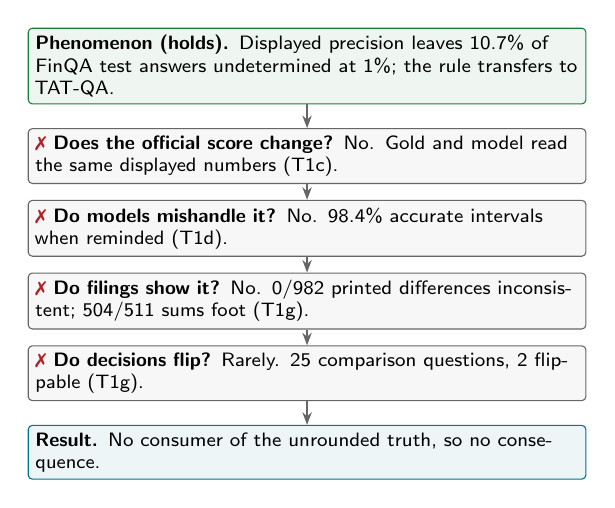
\begin{tikzpicture}[font=\sffamily\scriptsize,
  box/.style={draw=black!60, fill=black!3, rounded corners=1.5pt, align=left, text width=6.9cm, inner sep=2.6pt},
  arr/.style={-{Stealth[length=1.6mm]}, line width=0.6pt, black!60}]
\node[box, draw=cKeep, fill=cKeep!7] (p) {\textbf{Phenomenon (holds).} Displayed precision leaves 10.7\% of FinQA test answers undetermined at 1\%; the rule transfers to TAT-QA.};
\node[box, below=3mm of p] (l1) {\textcolor{failred}{\ding{55}} \textbf{Does the official score change?} No. Gold and model read the same displayed numbers (T1c).};
\node[box, below=2mm of l1] (l2) {\textcolor{failred}{\ding{55}} \textbf{Do models mishandle it?} No. 98.4\% accurate intervals when reminded (T1d).};
\node[box, below=2mm of l2] (l3) {\textcolor{failred}{\ding{55}} \textbf{Do filings show it?} No. 0/982 printed differences inconsistent; 504/511 sums foot (T1g).};
\node[box, below=2mm of l3] (l4) {\textcolor{failred}{\ding{55}} \textbf{Do decisions flip?} Rarely. 25 comparison questions, 2 flippable (T1g).};
\node[box, below=3mm of l4, draw=cConseq, fill=cConseq!7] (z) {\textbf{Result.} No consumer of the unrounded truth, so no consequence.};
\draw[arr] (p) -- (l1); \draw[arr] (l1) -- (l2); \draw[arr] (l2) -- (l3); \draw[arr] (l3) -- (l4); \draw[arr] (l4) -- (z);
\end{tikzpicture}
\caption{The consequence chain for the rounding line. Every link from the phenomenon to something a reader would act on was tested and found broken. The first link could have been read off the scorer before any experiment.}
\label{fig:chain}
\end{figure}

The same stage also exposed an untested assumption. The advisor's expected counts used a model in which each printed number is rounded independently; it predicted that about 25\% of printed differences would disagree with the difference of printed levels. The measured rate was 0 of 982. Filings are produced by a process that keeps tables consistent at the displayed precision---by computing from displayed values, by adjusting a line so the table foots, or both---so independent rounding is the wrong generative model for curated tables. Fifty tables, checked by hand before any expected count was published, would have shown this.

Stage C shows the same failure in a milder form. Its likely outcome was computable before it ran: the Gaussian overlap implied by a reliability near 0.97, which Stage B's rankings already suggested, is about 84\%, close to what was measured. A clean pass would have produced the stop rule ``use the reliability formula'', which is textbook \citep{spearman1910correlation,brown1910some}.

\subsection{Contributing factors}

\paragraph{Gates the data could not resolve.} Pre-registered gates were the best habit of the project, but two of them were set finer than the sample could resolve. In Stage B's confirmation, each recall check involved about 13 items, so one item moved recall by 7--8 points. Under a binomial model, even if the true per-item recall were 90\%, a single 13-item check would pass with probability 0.87 and eight such checks would all pass with probability about 0.32. The failed check (11/14) says little about the method. In Stage C, the tie groups at the positive 10\% boundary in the first five rounds were 12, 17, 11, 16 and 16 items against a limit of 20. A Poisson model with the observed mean gives a 40--70\% chance that at least one of eight rounds breaches the limit, before accounting for the scale's preference for round numbers. Both risks could have been computed from pilot data in minutes.

\paragraph{A gate on a parameter of the wrong model.} T3's only passing gate was a weight estimated inside a model that fit twice as badly as the additive alternative. A parameter gate should be read only after the model passes a fit check.

\paragraph{Questions chosen by the data at hand.} Stages A to D all used SEntFiN headlines because a cleaned copy and lexical baselines already existed. Convenience data pulled the questions toward subjective sentiment scores, which have no ground truth and no economic unit---precisely the property that made Stage B's reference unstable.

\paragraph{How agents behave under rules.} The student agents followed rules literally. In Stage A, an evidence gate that required per-row predictions from an older model, which no longer existed, blocked every experiment for nine rounds; the agents spent the time on proofs and on documentation that could be verified locally (manifests, checkers, reviews of reviews). Parallel task batches amplified sunk cost: by the time one task reported a null, its siblings had already built on the same premise.

\paragraph{Comparative advantage.} The author's edge is deep analysis. The FinQA rule is first-year numerical analysis---cancellation in a difference of nearly equal numbers \citep{higham2002accuracy}---and growth-rate rounding has long been studied in index-number practice \citep{gittings1991rounding}. Once the mathematics was easy, the paper had to compete on empirical novelty in a crowded field, where we were late.

\subsection{What worked}

Several habits made each ``no'' fast and believable, which is why three days were enough to reach a firm closeout. Gates and predictions were written down before data: the TAT-QA prediction was committed to the repository before any TAT-QA computation. Gates were not moved after the fact: 11/14 was not relabelled a pass, and the tie breach was not waived using the finer resolution of averaged scores. The project tried to kill its own best finding (T1b) and reported that it survived. Raw outputs, rejected versions and failed runs were kept, and the advisor recomputed every headline number from per-item records before ruling. None of this prevented the failure; all of it made the failure cheap to diagnose.

\section{What survives}
\label{sec:salvage}

\paragraph{A verified benchmark-precision note.} For financial QA with displayed inputs and a 1\% tolerance, a zero-parameter first-order rule predicts which questions the displayed precision cannot determine. On FinQA, 123 of 1,147 test questions (10.7\%) remain undetermined after duplicate disclosures, sum constraints and two independent AI semantic reviews (139 under the first review alone). On growth-rate questions the rule's prior prediction was 41.5\% against 40.5\% measured. Out of sample on TAT-QA, the frozen prediction was 24.5\% and the measurement 20.5\% (5,261 questions, 76\% of the arithmetic questions). Among these questions the sign of the answer is always determined; only its size is not.

\paragraph{A negative result about consequences.} This indeterminacy changes almost no official score (0.15\% of FinQA and 0.35\% of TAT-QA scored items, all explained by output digits). Filings are self-consistent at their displayed precision (0 of 982 printed differences inconsistent; 504 of 511 sum relations with zero residual), so independent-rounding probability models should not be used to estimate real rates.

\paragraph{Measurement facts for LLM scoring.} One model scoring financial headlines on a 0--100 scale has single-run reliability 0.975; its top-10\% list overlaps 84--87\% with an independent run and 91--92\% after averaging four runs, close to the Spearman--Brown prediction; same-batch scores are slightly more correlated than cross-batch scores. Ranking-based measurements of the same model were less stable in the tails.

\paragraph{Two small theoretical points.} In the tail-screening model, $\alpha=1$ does not imply a bounded widening factor, and per-stage exponents of a multi-stage screen cannot be multiplied without a joint or Markov condition; both have explicit counterexamples in the repository.

\section{Lessons: five questions before the first experiment}
\label{sec:lessons}

Table~\ref{tab:audit} lists, for each stage, the earliest signal that could have closed it and the cheapest test that would have read that signal. The times are our estimates and assume the test would have been read correctly; they are a hindsight bound, not a promise. Most of the project's three days, and more than 1,500 model sessions in the rounding line alone, went into questions that a few hours of reading could have answered.

\begin{table*}[!t]
\centering
\scriptsize
\renewcommand{\arraystretch}{1.18}
\begin{tabularx}{\textwidth}{@{}L{1.75cm}L{3.0cm}YYL{1.3cm}@{}}
\toprule
\textbf{Stage} & \textbf{What it cost} & \textbf{Earliest kill signal (when available)} & \textbf{Cheapest test that reads it} & \textbf{Test time} \\
\midrule
A. Certifiable FinLM & About a day; nine rounds; 125 unit tests & No consumer for the certified quantities; simple baselines matched by round 3. & Write the abstract with the strongest simple baseline beside it, and name who acts on the bound. & 1--2 h \\
B. Proxy tail (theory) & Derivations and a four-branch literature check & $\alpha=\rho^2$ in \citet{heffernan2004conditional}; LLM-cascade and proxy-selection work. & Targeted search on ``conditional extremes Gaussian'', ``LLM cascade copula'', ``proxy selection recall''. & 1 h \\
B. Proxy tail (measurement) & 64 scoring tasks & The reference disagreed with itself on the first 128-item pilot (1 shared item in two 10\% lists). & Compute gate power from pilot granularity before freezing the confirmation gate. & 15 min \\
C. Absolute scores & 250 calls, about 2 h & Predicted overlap from existing reliability; tie groups of 11--17 in early rounds. & Gaussian overlap from $r$; Poisson risk of a tie breach from pilot rounds. & 15 min \\
D. T3 & 92 calls & The passing gate lived in the worse-fitting model. & Fit check before the parameter gate. & 15 min \\
E. Rounding (T1c--T1g) & About 11 h; more than 1,500 model sessions & Gold programs and models read the same displayed numbers; filings foot at display precision. & Read the scorer; hand-check 50 printed differences; run the novelty check before T1d. & 1--2 h \\
\bottomrule
\end{tabularx}
\caption{Hindsight audit. For each stage: what it cost, the earliest signal that could have closed it, and the cheapest test that would have read the signal.}
\label{tab:audit}
\end{table*}

We condense the audit into five questions, to be answered in writing before the first experiment of any new line, and again at every fork.

\begin{enumerate}[leftmargin=1.3em]
\item \textbf{Who consumes the answer?} Name the score, decision or price that changes if the hypothesis is true. For a benchmark defect, read the scorer and check that the defect passes through it. If nothing changes, stop.
\item \textbf{Has it been done?} Spend two hours on prior art, including the last twelve months of preprints and code repositories, and have someone other than the proposer search. ``I did not find it'' does not count as novel.
\item \textbf{What is the cheapest kill test, and does it run first?} Write down the result that would end the line and run that test before anything that scales.
\item \textbf{Can the instrument resolve the gate?} From pilot data, compute granularity, tie mass and the probability that the gate passes under a plausible truth. Do not pre-register a gate the sample cannot resolve.
\item \textbf{Is our edge decisive here?} If the mathematics is textbook and the empirical field is crowded, expect to lose the race to novelty.
\end{enumerate}

Two further rules address the agent setting specifically. Validate every generative assumption on about fifty real cases before using it to produce expected counts. And when agents execute, give the advisor a budget for reading and thinking that is not smaller than the budget for running: the bottleneck was never execution.

For a reader facing a similar question---``does some property of a benchmark's inputs make its answers uncertain?''---the cheapest path is: read the scorer to see whether the property reaches the score; search the last year of benchmark audits for the same dataset; hand-check fifty items; and only then count.

\section*{Limitations}

This is a post-mortem written with hindsight, which makes early signals look clearer than they were. The time estimates in Table~\ref{tab:audit} assume the cheap tests would have been read correctly. All semantic reviews and adjudications were done by AI models from a single vendor, with no human spot-check and no cross-vendor replication; the counts that depend on them (139, 123, and the attribution of rejections) carry that limitation. Benchmark data are public, so training exposure of the evaluated models cannot be ruled out. Finally, the analysis was drafted by the same advisor whose direction failed, which is a conflict of interest; we have tried to state its errors plainly, and the full record is public so others can judge.

\section*{Use of AI}

The research was directed by an LLM advisor (Claude) and executed by LLM agents (OpenAI Codex with GPT-family models), as described in \S\ref{sec:setting}. This report was drafted with Claude from the repository's records; the author is responsible for its content.

\section*{Data and code}

All task briefs, prompts, raw model outputs, analysis code, pre-registered protocols and reviews are at \url{https://github.com/130U/proxy-tail}. The state of the repository at the moment of closeout, before translation into English, is preserved under the tag \texttt{closeout-2026-11-17}.

\bibliography{references}

\appendix

\section{Timeline}
\label{app:timeline}

Times are from the repository's commit log (US Eastern).

\begin{table}[H]
\centering
\scriptsize
\begin{tabular}{@{}ll@{}}
\toprule
\textbf{When} & \textbf{Event} \\
\midrule
Nov 15 & Stage A begins (separate workspace) \\
Nov 16 & Stage A closes after nine rounds \\
Nov 16 & Stage B: theory, lexical analysis, 64 scoring tasks \\
Nov 16, 07:16 & Repository started; Stage B imported \\
Nov 16, 08:55--10:56 & Stage C: absolute-score replication \\
Nov 16, 21:15 & Four one-day probes issued (T1--T4) \\
Nov 16, 21:36 & T1 finds 196/1,147 \\
Nov 16, 21:56 & T3 complete \\
Nov 16, 22:56 & T1a complete (law) \\
Nov 16, 23:10 & T1b complete (139 survive) \\
Nov 17, 00:27 & T1c complete (no effect on scores) \\
Nov 17, 06:23 & T1d complete (models know when asked) \\
Nov 17, 07:52 & T1f complete (4 of 5 candidates have prior work) \\
Nov 17, 08:31 & T1g prediction committed \\
Nov 17, 08:52 & T1g complete (no consequence) \\
Nov 17, 09:21 & Closeout \\
\bottomrule
\end{tabular}
\caption{Timeline of the project.}
\end{table}

\section{Key numbers for the rounding line}
\label{app:numbers}

\begin{table}[H]
\centering
\scriptsize
\renewcommand{\arraystretch}{1.12}
\begin{tabular}{@{}L{1.1cm}L{5.7cm}@{}}
\toprule
\textbf{Step} & \textbf{Result} \\
\midrule
T1 & 196/1,147 FinQA test questions (17.1\%) have a witness outside the 1\% tolerance inside the inputs' rounding box. \\
T1a & $R=(1+g/2)/(\Delta-|g|/2)$ exact on 1,411 canonical growth questions; first-order rule agrees with exact classification on 5,337 questions; prior prediction 41.5\% vs.\ 40.5\% measured. \\
T1b & 511 sum relations and 21 duplicate disclosures rescue 1 question; 56 more removed by semantic review; 139 (12.1\%) remain. \\
T1c & 392 questions in independent sessions; error gap witness vs.\ control +5.1 pp (CI includes 0); 0 of 68 rejections due to input precision alone. \\
T1d & Unprompted: printed digits vs.\ true reliable digits, Spearman 0.02; 61.6\% over-report by more than one digit. Reminded: 98.4\% intervals accurate, 99.7\% correct 1\% calls. Second review: 139 $\to$ 123 (both reviews valid), 132 by majority; $\kappa=0.76$ on verdicts, $\kappa=0.88$ on rejection attributions. \\
T1f & Candidates 2--5 have prior work; candidate 1 (rule and count) not found in the literature searched. \\
T1g & 0/982 printed differences inconsistent (25\% predicted); 7/511 sums with non-zero residual; affected scores 5/3,265 (FinQA) and 16/4,524 (TAT-QA); 25 comparison questions, 2 flippable; TAT-QA prediction 24.49\% vs.\ 20.47\% measured; 154 same-fact pairs at two precisions, 18 of 96 substitutions move the answer by more than 1\%. \\
\bottomrule
\end{tabular}
\caption{Main numbers of the rounding line. Full records are in \texttt{research/t1*} in the repository.}
\end{table}

\section{Repository map}
\label{app:repo}

\begin{table}[H]
\centering
\scriptsize
\begin{tabular}{@{}L{2.4cm}L{4.4cm}@{}}
\toprule
\textbf{Path} & \textbf{Contents} \\
\midrule
\texttt{report/} & This report (PDF and LaTeX source) \\
\texttt{tasks/} & Every task brief, in the order issued \\
\texttt{research/} & One folder per stage or task; see \texttt{research/README.md} \\
\texttt{source\_materials/} & Snapshot of the earlier project and source audits \\
\texttt{archive/} & Historical homepages, roadmap and the stale paper draft \\
\bottomrule
\end{tabular}
\caption{Where to find the material.}
\end{table}

\end{document}
